\documentclass{beamer}

\usepackage{biblatex}
\bibliography{bibliography}
\AtBeginBibliography{\small}
\usepackage{hyperref}
\usepackage{siunitx}

\usetheme{Antibes}
\usecolortheme{beaver}

\title{Bearing Condition Monitoring}
\subtitle{Quadro Teorico}
\author{Sergio Vanegas}
\institute{Modelway S.r.l.}
\date{\today}

\begin{document}

\frame{\titlepage}

\begin{frame}{Table of Contents}
    \tableofcontents
\end{frame}

\section{Introduzione}

\begin{frame}{Oggetto dell'intervento}
    \begin{itemize}
        \item SKF: uno dei leader mondiali nel settore bearing.
        \item La failure/anomaly detection dei cuscinetti risulta importante per:
        \begin{itemize}
            \item Rilevamento di situazioni pericolose.
            \item Implementazione della manutenzione programata e preventiva.
        \end{itemize}
        \item Goal: fornire a SKF un tool software che rilevi automaticamente la presenza di failure o anomalie sul cuscinetto.
    \end{itemize}
\end{frame}

\section{Pre-analisi}

\begin{frame}[allowframebreaks]{Analisi ad Elementi Finiti}
    Forti stress multiassiali sui contatti delle piste interne ed esterne governati dalla teoria di Hertz.

    \begin{figure}
        \centering
        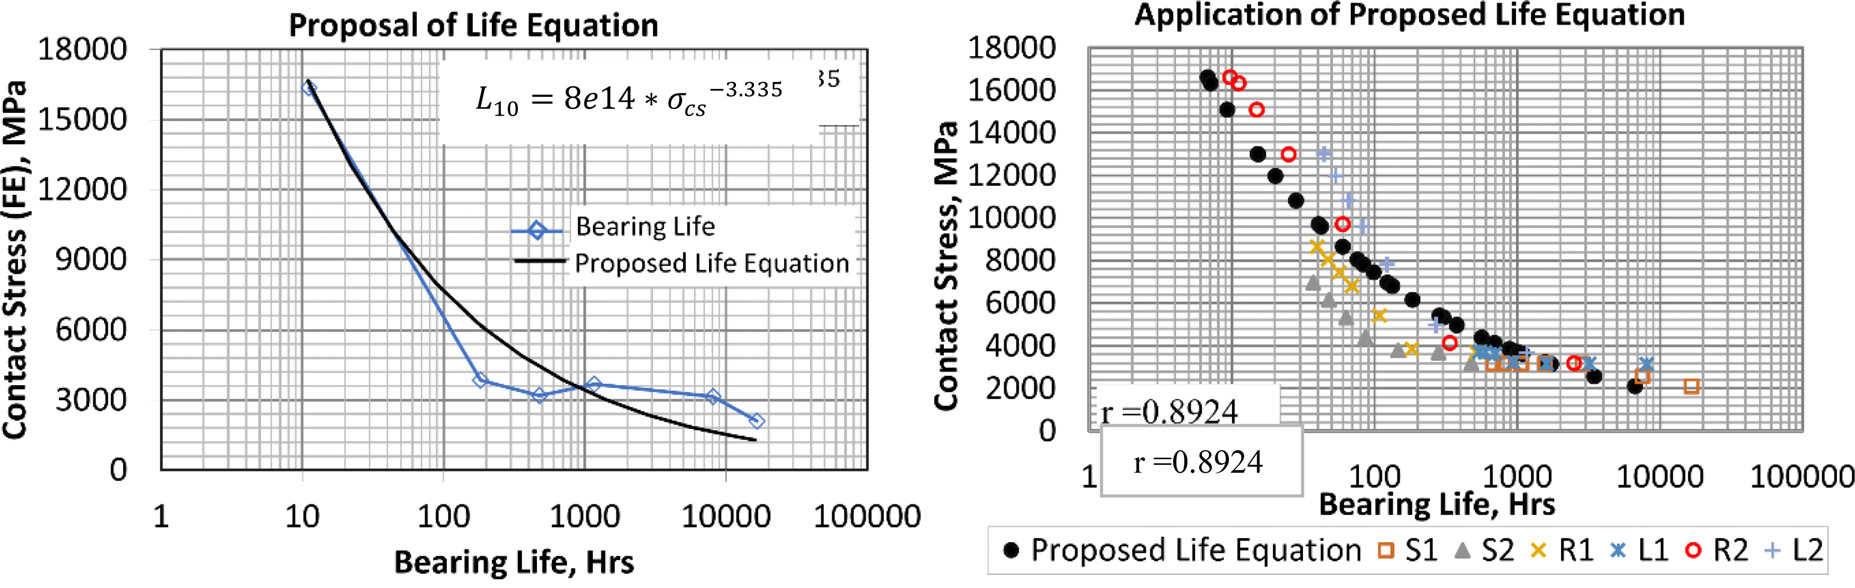
\includegraphics[width=\textwidth]{Figures/FE_Life_Curve.png}
        \caption{Relazione tra la vita del cuscinetto e lo stress medio di contatto}
        \label{fig:FE_Life_Curve}
    \end{figure}

    \framebreak

    \begin{itemize}
        \item Modellazione FE (simmetrica) con imposizione di duty cycle\cite{raju2018bearing}.
        \item I cuscinetti si guastano tipicamente a causa della Rolling Contact Fatigue (sotto la superficie).
        \item Buona correlazione tra ``FE contact stress'' e la vita utile dei cuscinetti.
        \item Modello adattato modificando:
        \begin{itemize}
            \item La distribuzione del duty cycle.
            \item I fattori di rugosità superficiale/microgeometria.
        \end{itemize}
    \end{itemize}
\end{frame}

\begin{frame}[allowframebreaks]{Analisi del pre-carico}
    Sulla base del modello matematico e dello spettro di carico, viene calcolata e stimata la durata dell'unità cuscinetto del mozzo della ruota\cite{niu2014life}.

    \begin{figure}
        \centering
        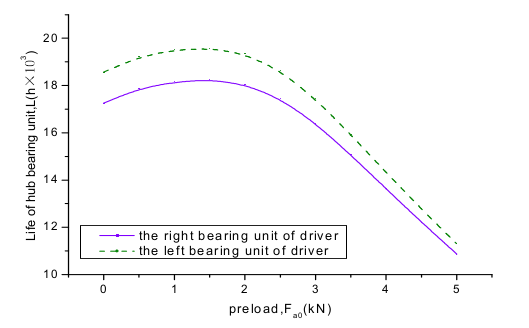
\includegraphics[width=0.5\textwidth]{Figures/Preload_Life_Estimation.png}
        \caption{Relazione tra pre-carico e vita utile}
        \label{fig:Preload_Life_Curve}
    \end{figure}
    
    Dall'altra parte, la frequenza naturale del cuscinetto aumenta con la forza di pre-carico (questa tendenza tende a rallentare).

    \begin{figure}
        \centering
        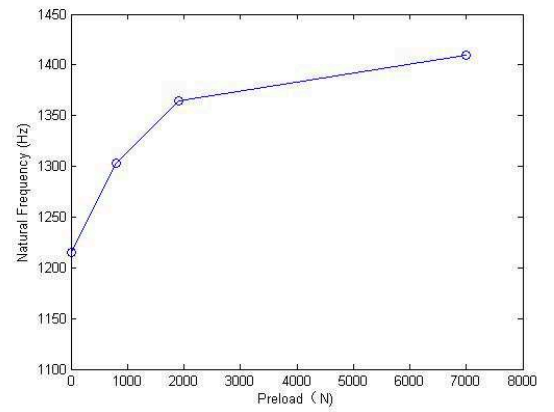
\includegraphics[width=0.4\textwidth]{Figures/Preload_NatFreq.png}
        \caption{Relazione tra pre-carico e frequenza naturale}
        \label{fig:Preload_Freq}
    \end{figure}

    Questo significa che si può stabilire una relazione tra la frequenza naturale del cuscinetto e la sua vita utile.
\end{frame}

\section{Monitoraggio}

\begin{frame}[allowframebreaks]{Frequenze delle vibrazioni}
    \begin{itemize}
        \item Descomposizione del segnale\cite{tang2019fault}:
        \begin{itemize}
            \item Frequenze del cuscinetto.
            \item Frequenze dei difetti.
            \item Frequenze del rumore.
        \end{itemize}
        \item Analisi statistica dello spettro\cite{xue2022fault}:
        \begin{itemize}
            \item Descomposizione tramite \textit{Resonance-based Signal Sparse Decomposition} (RSSD).
            \begin{itemize}
                \item Risonanza trovata utilizzando \textit{Tunable Q-factor Wavelet Transform} (TQWT).
            \end{itemize}
            \item Metodo di estrazione della frequenza di difetto basato su Ration of Smoothness and Kurtosis (RSK).
        \end{itemize}
        \framebreak
        \item Analisi diretto dello spettro basata su STFT\cite{rubio2012experimental}.
    \end{itemize}
    
    \begin{figure}
        \centering
        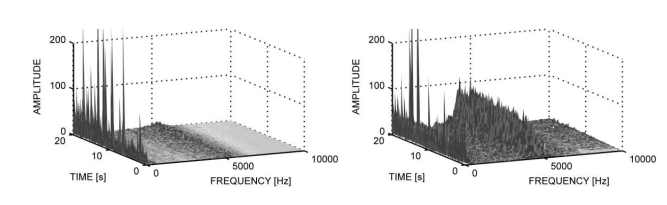
\includegraphics[width=0.8\textwidth]{Figures/STFT.png}
        \caption{STFT delle vibrazioni (cuscinetto buono/danneggiato)}
        \label{fig:STFT}
    \end{figure}
\end{frame}

\begin{frame}{Carica multiassiale della ruota}
    \small
    È possibile stabilire una legge per determinare quando sostituire i cuscinetti in funzione dell'equilibrio delle forze\cite{zhao2021service}.

    \begin{figure}
        \centering
        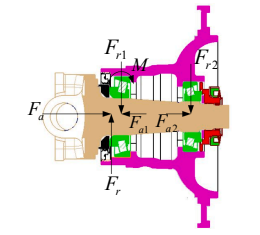
\includegraphics[width=0.3\textwidth]{Figures/Force_Diagram.png}
        \caption{Schema delle forze sul cuscinetto del mozzo ruota}
        \label{fig:Forces_Bearing}
    \end{figure}

    Contando il ciclo di distribuzione combinato dei carichi multiassiali e classificando i tipi di carica, la vita utile del cuscinetto è calcolata in base al \textbf{carico di contatto circonferenziale} del cuscinetto.
\end{frame}

\begin{frame}{Rumore acustico}
    Analisi del segnale basata sull'autocorrelazione in tempo discreto.

    \begin{figure}
        \centering
        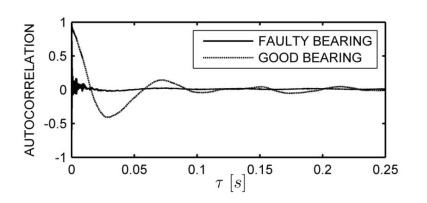
\includegraphics[width=0.6\textwidth]{Figures/Acoustic.png}
        \caption{Autocorrelazione del rumore acustico ($f_s = \SI{20}{\kilo \hertz}$)}
        \label{fig:acoustic}
    \end{figure}

    Anche se l'ambiente non è ideale per l'analisi del rumore acustico, la caratterizazione delle frequenze del cuscinetto e dei difetti può essere usata per calibrare un filtro Band-Pass.

\end{frame}

\section*{Bibliografia}

\begin{frame}[allowframebreaks]{Bibliografia}
    \printbibliography
\end{frame}

\end{document}